\documentclass[hidelinks]{article}
\usepackage{amsmath, amssymb, amsthm}
\usepackage{thmtools}
\usepackage{algorithm}
\usepackage{algpseudocode}
\usepackage{nameref, hyperref, cleveref}
\usepackage{tikz}
\usepackage[shortlabels]{enumitem}
\usepackage{todonotes}
\usepackage{enumitem}

\usepackage[left=2.2in, right=1.25in, marginparwidth=1.7in]{geometry}

\reversemarginpar

\setenumerate{itemsep=-.5ex}

\usetikzlibrary{positioning, arrows.meta, shapes}

\newcommand{\Ac}{\mathcal{A}}  % alphabet
\newcommand{\Lc}{\mathcal{L}}  % label function
\newcommand{\Gc}{\mathcal{G}}  % labeled graph
\newcommand{\Hc}{\mathcal{H}}  % labeled graph
\newcommand{\Vc}{\mathcal{V}}
\newcommand{\Ec}{\mathcal{E}}
\newcommand{\Bc}{\mathcal{B}}
\newcommand{\Kc}{\mathcal{K}}
\newcommand{\Fc}{\mathcal{F}}
\newcommand{\Fs}{\mathsf{F}}
\newcommand{\GtH}{{\Gc^\to\Hc}}
\newcommand{\shift}[1]{\mathsf{X}_{#1}}
\newcommand{\term}[1]{\textit{#1}}
\newcommand{\Sync}{\textsf{Sync}}
\newcommand{\GI}{\textsf{GI}}
\newcommand{\LGI}{\textsf{LGI}}

\usepackage[bitstream-charter, cal=cmcal]{mathdesign}

\theoremstyle{definition}
% \newtheorem{theorem}{Theorem}
\declaretheorem[numberwithin=section]{theorem}
\declaretheorem[sibling=theorem]{lemma}
\declaretheorem[sibling=theorem]{definition}
\declaretheorem[sibling=theorem]{corollary}
% \newtheorem{definition}{Definition}
% \newtheorem{lemma}{Lemma}

\renewcommand{\baselinestretch}{1.2}
\setlength{\parskip}{.05em}

\title{Computational complexity for presentations of sofic shifts}
\author{Justin Cai}

\begin{document}

\maketitle

\begin{abstract}
    Given an irreducible presentation of a sofic shift, it is well known that the 
    shift it presents is irreducible and that there is a 
    procedure that yields the unique vertex-minimal presentation for
    this shift in polynomial time. However, if one was given a reducible 
    graph, there is not necessarily a unique vertex-minimal presentation, and 
    a procedure for the construction of some minimal presentation in 
    this case is unknown. It can be the case where the presentation still presents 
    an irreducible shift, but the previous procedure will not produce the 
    minimal presentation. In this thesis, we show complexity results around 
    these problems.
\end{abstract}

% \todo[inline]{Figure out correct theorem referencing.}

\section{Preliminaries}

\begin{definition}
    Let \(\Ac\) be a finite set. The \term{full \(\Ac\)-shift} is the set \(\Ac^\mathbb{Z}\) of all 
    bi-infinite sequences over \(\Ac\) (i.e. functions from \(\mathbb{Z}\) to \(\Ac\), hence the 
    usual notation for the set of all functions from \(\mathbb{Z}\) to \(\Ac\)).
\end{definition}

\noindent A \term{block} (or \term{word}) is a finite sequence of letters over some alphabet \(\Ac\). 
Let \(x=(x_i)_{i \in \mathbb{Z}}\) be a bi-infinite sequence. For \(i \leq j\), the block from the 
\(i\)th coordinate to the \(j\)th coordinate is denoted \[x_{[i,j]} \triangleq x_i x_{i+1} \dots x_{j}.\]

\begin{definition}
    Let \(\Fc\) be a set of words over some alphabet. A \term{subshift} is a subset \(\shift{\Fc}\)
    of some full shift \(\Ac^\mathbb{Z}\) such that no word in \(\Fc\) appears in any point of the subshift,
    defined as
    \[\shift{\Fc} \triangleq \Big\{ \; (x_i)_{i \in \mathbb{Z}} \in \Ac^\mathbb{Z} \; : \; \forall i, j \in \mathbb{Z}, i\leq j \quad  x_{[i,j]} \notin \Fc \; \Big\}.\]
\end{definition}

\begin{definition}
    A \term{graph} \(G\) is a \(4\)-tuple \(G = (\Vc, \Ec, i, t)\), where \(\Vc\) is a finite 
    set of \term{vertices}, \(\Ec\) is a finite set of \term{edges}, and \(i : \Ec \to \Vc\) and 
    \(t : \Ec \to \Vc\) are functions assigning an \term{initial} and \term{terminating} vertex for 
    each edge, respectivley. For an arbitrary graph \(G\), let 
    \(\Vc_G\), \(\Ec_G\), \(i_G\), and \(t_G\) denote the graph's vertices, edges, and 
    intial and terminating vertex functions, respectivley. If the choice 
    of \(G\) is understood, then the subscripts will be dropped for notational convenience.

    For \(I \in \Vc\), the \term{outgoing edges of \(I\)} is the set of edges starting at \(I\),
    denoted 
    \[i^{-1}(I) \triangleq \{e \in \Ec : i(e) = I\}.\]
    Similary, the \term{incoming edges of \(I\)} is the set of edges terminating at \(I\), 
    denoted
    \[t^{-1}(I) \triangleq \{e \in \Ec : t(e) = I\}.\]

    A graph is \term{essential} if all vertices have at least one incoming and outgoing edge;
    i.e. for all \(I \in \Vc\), \(i^{-1}(I) \ne \varnothing\) and \(t^{-1}(I) \ne \varnothing\).

\end{definition}

\begin{definition}
    A \term{labeled graph} \(\Gc\) is a pair \(\Gc = (G, \Lc)\), where \(G\) is a graph and \(\Lc : \Ec \to \Ac\) is the 
    \term{labeling function} from the edges of \(G\) onto some finite alphabet \(\Ac\).

    A labeled graph is \term{deterministic} if for each vertex, the labels of the outgoing edges at that vertex are all distinct 
    (i.e. \(\Lc|_{i^{-1}(I)}\) is injective for all \(I \in \Vc\)).
\end{definition}

\begin{definition}
    Let \(G\) be a graph. The \term{edge shift of \(G\)} is the set \(\shift{\Gc}\) of all bi-infinite 
    paths on \(G\), defined as 
    \[\shift{G} \triangleq \Big\{ \; (x_i)_{i \in \mathbb{Z}} \in \Ec^\mathbb{Z} \; : \; \forall i \in \mathbb{Z} \quad t(x_i) = i(x_{i+1}) \; \Big\}. \]
\end{definition}

\noindent As a consequence of this definintion, \(\Bc(\shift{G})\) is the 
set of all finite paths \todo{Define paths.} on \(G\), so elements of \(\Bc(\shift{G})\) are called
\term{paths on \(G\)}. \todo{Only if \(G\) is essential. Otherwise, if \(G\) 
is not essential, then there can be paths not in \(\Bc(\shift{G})\).}


\begin{definition}
    Let \(\Gc = (G, \Lc)\) be a labeled graph. The \term{presentation of \(\Gc\)} is the set \(\shift{\Gc}\)
    of the labels of all bi-infinite paths from \(\shift{G}\), defined as the image of 
    \(\shift{G}\) under \(\Lc_\infty\):
    \todo{Define sliding block codes so \(\Lc_\infty\) makes sense.}
    \[\shift{\Gc} \triangleq \Lc_\infty(\shift{G}).\]
    We say a word \(w \in \Bc(\shift{\Gc})\) is \term{presented by a path} \(\pi \in \Bc(\shift{G})\) if \(\Lc(\pi) = w\).
\end{definition}

\begin{definition}
    Let \(\Gc = (G, L)\) be a labeled graph. For a vertex \(I \in \Vc_\Gc\), the 
    \term{follower set of \(I\)} is the set 
    \[F(I) \triangleq \big\{ \Lc(\pi) : \pi \in \Bc(\shift{G}), i(\pi) = I \big\}.\]
    For a word \(w \in \Bc(\shift{\Gc})\), the \term{follower set of \(w\)}
    is the set 
    \[F(w) \triangleq \big\{ u \in \Bc(\shift{\Gc}) : wu \in \Bc(\shift{\Gc})\big\}\]
\end{definition}

\begin{definition}
    Let \(\Gc = (G, \Lc)\) be a labeled graph, \(I\) be some vertex in \(\Gc\), and \(w \in B(\shift{\Gc})\).
    If every path \(\pi\) in \(\Gc\) that presents \(w\) ends at \(I\), then we say \term{\(w\) synchronizes to \(I\)}.
    We say that \(w\) is \term{synchronizing for \(\Gc\)} if it synchronizes to some vertex in \(\Gc\). 
    If there is a word that synchronizes to \(I\), then we say that the vertex \term{\(I\) is synchronizing}.
    Finally, we denote 
    \(S(\Gc)\) as the set of all syncrhonizing words for \(\Gc\).
    % A word \(w \in \Bc(\shift{\Gc})\) is 
    % synchronizing if for all paths \(\pi\) in \(\Gc\) that present \(w\) end at the 
    % same vertex. A vertex \(I \in \Vc_\Gc\) is synchronizing if there is a word \(w\) such 
    % that all words that present \(w\) end at \(I\). 
\end{definition}

Let \(\Gc\) be a deterministic labeled graph. It follows that for every vertex \(I\) in \(\Gc\)
and every \(w \in F(I)\), there is a unique path labeled \(w\) starting at \(I\). We can 
define a partial \term{transition function} \(\delta_\Gc : \Vc_\Gc \times \Ac_\Gc^* \to \Vc_\Gc\) 
\todo{Define \(\Ac_\Gc\).}
with \(\delta_\Gc(I, w) \triangleq t(\pi)\) if there is a path \(\pi\) labeled \(w\) starting 
at \(I\). If \(w = \Lc(\pi)\) and \(\Lc(\tau)\) for paths \(\pi\) and \(\tau\), then by 
determinism, \(\pi = \tau\) so \(t(\pi) = t(\tau)\), so this function is well defined.
It will be useful to make \(\delta_\Gc\) total by first defining \(\Vc_\Gc^0 \triangleq \Vc_\Gc \cup \{0\}\),
where \(0\) is a constant distinct from \(\Vc_\Gc\). Then, by extending the domain of \(\delta_\Gc\) to 
\(\Vc_\Gc^0 \times \Ac_\Gc^*\) and the codomain to \(\Vc_\Gc^0\), define \(\delta_\Gc(I, w) \triangleq 0\) 
if \(w \notin F(I)\) and \(\delta_\Gc(0, w) = 0\). Finally, define 
the \term{subset transition function} \(\Delta_\Gc : \mathcal{P}(\Vc) \times w \to \mathcal{P}(\Vc)\)
with \(\Delta_\Gc(S, w) \triangleq \{ \delta_\Gc(I, w) : I \in S \text{ and } \delta_\Gc(I, w) \neq 0\}\).

\begin{theorem}
    Let \(\Gc\) be a deterministic labeled graph, and \(I\) be a vertex in \(\Gc\). The following properties of the 
    transition function are true:

    \begin{enumerate}[(i)]
        \item \(w \in F(I)\) if and only if \(\delta_\Gc(I, w) \neq 0\)
        \item \(w \in \Bc(\shift\Gc)\) if and only if \(\Delta_\Gc(\Vc_\Gc, w) \neq \varnothing\)
        \item \(w\) synchronizes to \(I\) if and only if \(\Delta_\Gc(\Vc_\Gc, w) = \{I\}\)
    \end{enumerate}
\end{theorem}

\begin{definition}
    Let \(\Gc\) be an essential labeled graph. The \term{\(\Gc\) kill state graph with alphabet \(\Ac\)}
    is the labeled graph \(\Gc^0\) taking the same vertices and edges as \(\Gc\) with 
    an additional vertex \(0\) and edges such that for each \(a \in \Ac\) and vertex \(I\) in \(\Gc\),
    if there is no edge starting at \(I\) labeled \(a\), then there is an edge in \(\Gc^0\) 
    between \(I\) and \(0\) labeled a.
\end{definition}

\begin{definition}
    Let \(\Gc\) and \(\Hc\) be labeled graphs. The \term{label product of \(\Gc\) and \(\Hc\)}
    is the labeled graph \(\Gc * \Hc\) such that if there is an edge \(e_1\) in \(\Gc\)
    between \(I_1\) and \(J_1\) and an edge \(e_2\) in \(\Hc\) between \(I_2\) and \(J_2\)
    with \(\Lc_\Gc(e_1) = \Lc_\Hc(e_2)\), then there is an edge in \(\Gc * \Hc\) between 
    \((I_1, I_2)\) and \((J_1, J_2)\) labeled \(\Lc_\Gc(e_1) = \Lc_\Hc(e_2)\). That is, 
    \begin{align*}
        \Vc_{\Gc * \Hc} &\triangleq \Vc_\Gc \times \Vc_\Hc \\ 
        \Ec_{\Gc * \Hc} &\triangleq \{ (e_1, e_2) \in \Ec_\Gc \times \Ec_\Hc\ : \Lc(e_1) = \Lc(e_2)\} \\ 
        i_{\Gc * \Hc}(e_1, e_2) &\triangleq (i_\Gc(e_1), i_\Gc(e_2)) \\ 
        t_{\Gc * \Hc}(e_1, e_2) &\triangleq (t_\Hc(e_1), t_\Hc(e_2)) \\ 
        \Lc_{\Gc * \Hc}(e_1, e_2) &\triangleq \Lc_\Gc(e_1) \qquad ( = \Lc_\Hc(e_2) )
    \end{align*}
\end{definition}

\begin{theorem}
    If there is a path in \(\Gc * \Hc\) labeled \(w\) starting at \((I, J)\), then 
    there is a path in \(\Gc\) labeled \(w\) starting at \(I\) and a path in \(\Hc\)
    labeled \(w\) starting at \(J\).
\end{theorem}

\todo[inline]{Add theorem showing that \(\shift{G}\) and \(\shift{\Gc}\) are shift spaces.}
\todo[inline]{Add theorem showing that shift spaes are uniquely defined by a language.}

% \section{Basic properties of sofic shifts}

% \todo[inline]{Irreducible presentations, synchronizing presentations}

% \begin{theorem}
%     Let \(\Gc = (G, \Lc)\) be a labeled graph and \(\pi\) be a path in \(\Gc\). If \(\Lc(\pi)\)
%     is synchronizing, then \(F(\Lc(\pi)) = F(t(\pi))\).
% \end{theorem}

% \begin{theorem}
%     If \(F(\Lc(\pi)) = F(t(\pi))\), then \(\Lc(\pi)\) is synchronizing.
% \end{theorem}

\section{Irreducibility}

\noindent Consider the reducible graph \(\Gc\):

\begin{figure}[h]
    \centering
    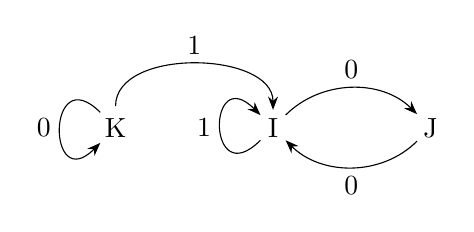
\begin{tikzpicture}
        [vertex/.style={circle, radius=10mm, inner sep=1pt},
         shorten <=1pt, shorten >= 1pt, >={Stealth[]}]
        \node[vertex] (A) at (0,0) {I};
        \node[vertex] (B) at (2,0) {J};
        \node[vertex] (C) at (-2, 0) {K};

        \path [->] (A) edge[out=225, in=135, distance=10mm] node[left] {$1$} (A);
        \path [->] (A) edge[out=45, in=135] node[above] {$0$} (B);
        \path [->] (B) edge[out=225, in=-45] node[below] {$0$} (A);
        \path [->] (C) edge[out=90, in=90] node[above] {$1$} (A);
        \path [->] (C) edge[out=135, in=225, distance=10mm] node[left] {$0$} (C);
    \end{tikzpicture} 
\end{figure}

\noindent The shift that subgraph induced by \(I\) and \(J\) is the even shift, and every 
word presented by a path starting from \(K\) is presented by some path starting at 
\(I\) and \(J\). Hence, this graph presents the even shift. Additionly, it is 
also follower-separated as \(01 \in F(K)\backslash F(I)\), \(1 \in F(K)\backslash F(J)\),
and \(1 \in F(I) \backslash F(J)\). 

When do follower-separated reducible graphs present irreducible shifts? We will first look 
at a simple class of reducible graphs.

Let \(\GtH\) be an essential, deterministic, follower-separated graph with two irreducible components
that induce two subgraphs, namely \(\Gc\) and \(\Hc\), such that there is 
exactly one edge starting in \(\Gc\) and ending in \(\Hc\). 
Some properties of \(\GtH\) are that the vertices of \(\Gc\) and \(\Hc\)
partition the vertices of \(\GtH\), both \(\Gc\) and \(\Hc\) are essential,  
any vertex in \(\Hc\) is reachable from any vertex in \(\GtH\), and no vertex in \(\Gc\) 
is reachable from any vertex in \(\Hc\).

% Let \(\Gc=(G, \Lc_\Gc)\) and \(\Hc = (H, \Lc_\Hc)\) be irreducible, follower-separated
% graphs.
% Fix two vertices, \(I \in \Vc_\Gc\) and \(J \in \Hc\), and some label \(\ell\) 
% not in the outgoing labels of \(I\) (i.e. \(\ell \notin \Lc_\Gc(i^{-1}(I))\)). Define the graph 
% \(\GtH = (G^\to H, \Lc_{\GtH})\) be the disjoint union of \(\Gc\) and \(\Hc\) plus one
% distinct edge \(e\) with \(i(e) = I\), \(t(e) = J\), and \(\Lc(e) = \ell\).

% Some immediate properties of \(\GtH\) are that the graph is deterministic \(\shift{\Gc} \subseteq \shift{\GtH}\),
% \(\shift{\Hc} \subseteq \shift{\GtH}\), and that there exists a path from any 
% vertex in \(\GtH\) to any vertex in \(\Hc\).

\begin{figure}[h]
    \centering
    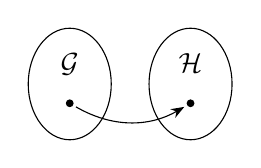
\begin{tikzpicture}[graph/.style={shape=ellipse, draw, minimum width=3em, text depth=1.5em},
                        dot/.style={shape=circle, fill, inner sep=1pt}]
        \node[graph] (G) at (0,0) {\(\Gc\)};
        \node[graph, right=of G] (H) at (0,0) {\(\Hc\)};
        \node[dot,below=-1.5em of G] (I) {};
        \node[dot,below=-1.5em of H] (J) {};
        \path [->] (I) edge[bend right, shorten <=1pt, shorten >= 1pt, >={Stealth[]}] node[above] {} (J);
    \end{tikzpicture}
    \caption{Representation of \(\GtH\).}
\end{figure}

\begin{theorem}\label{extensionthm}
    \todo{Related to a comment below, but this is just a corollary of [Lind and Marcus 3.3.16]
    and the nature of \(\GtH\)}
    Every word \(u \in \Bc(\shift{\GtH})\) can be extended on the right to a 
    word \(u w \in \Bc(\shift{\GtH})\) that syncrhonizes to a vertex \(I\) in \(\Hc\).
\end{theorem}

\begin{proof}
    Let \(u \in \Bc(\shift{\GtH})\). As \(\GtH\) is deterministic and 
    follower-separated, then by [Lind and Marcus 3.3.16], we can 
    extend \(u\) on the right to \(uw \in \Bc(\shift{\GtH})\) so that \(uw\)
    synchronizes to some vertex \(J\). As \(I\) is a vertex in \(\Hc\), 
    \(I\) can be reached from \(J\), so let \(v\) be  the label of a path 
    from \(I\) to \(J\). Then, \(uwv \in \Bc(\shift{\GtH})\) and any path presenting 
    \(uwv\) must end at \(J\), so \(uwv\) synchornizes to \(I\).
\end{proof}

\begin{corollary}\label{hsync}
    Every vertex in \(\Hc\) is synchronizing for \(\GtH\). 
\end{corollary}

\begin{proof}
    For a vertex \(I\) in \(\Hc\), take any word \(u \in \Bc(\shift{\GtH})\) and
    use \Cref{extensionthm} to synchronize it to \(I\). Hence, there is a word that synchronizes 
    to \(I\), so \(I\) is synchronizing.
\end{proof}

\begin{lemma}\label{wordlemma}
    Let \(u \in \Bc(\shift{\GtH})\). If \(u \notin \Bc(\shift{\Hc})\), then \(\shift{\GtH}\) is 
    reducible.
\end{lemma}

\begin{proof}
    By \Cref{extensionthm}, we can extend \(u\) on the right to a word \(uw \in \Bc(\shift{\GtH})\)
    so that any path presenting \(uw\) ends at some vertex \(I\) in \(\Hc\). Hence, for any word \(v \in F(uw)\), a 
    path presenting \(uwv\) ends at some vertex in \(\Hc\), so \(F(uwv) \subseteq \Bc(\shift{\Hc})\)
    \todo{Probably will expand this later. Argue that \(uwv\) is synchronizing, so \(F(uwv) = F(J)\)
    for some vertex \(J\) in \(\Hc\), so \(F(uwv) = F(J) \subseteq \bigcup_{K \in \Vc_\Hc} F(K) = \Bc(\shift{\Hc})\)}. 
    As \(u \notin \Bc(\shift{\Hc})\), we have \(u \notin F(uwv)\). Thus, there is no word in 
    \(\Bc(\shift{\GtH})\) joining the word \(uw\) and \(u\), so \(\shift{\GtH} \) is reducible.
\end{proof}

% \begin{theorem}
%     If \(\shift{\GtH}\) is irreducible, then \(\ell \in \Lc(t^{-1}_H(J))\).
%     % and for all \(w \in B(\shift{\Gc})\),
%     % \(w\ell \in B(\shift{\GtH})\) implies \(w\ell \in B(\shift{\Hc})\).
% \end{theorem}

% \begin{proof}
%     Suppose \(\ell \notin \Lc(t^{-1}_H(J))\). Considering just \(\Hc\), 
%     if \(\ell \in \Bc(\shift{\Hc})\), then a path presenting \(\ell\) does not 
%     end at \(J\). As \(\Hc\) is follower-separated, there is a word 
%     \(w \in F(J)\) and \(w \notin F(K)\) for all \(K \in \Vc_\Hc \backslash \{J\}\). 
%     \todo{This assumption is incorrect.}
%     Hence, we have \(\ell w \in \Bc(\shift{\GtH})\) but \(\ell w \notin \Bc(\shift{\Hc})\), 
%     so by Lemma 1, \(\shift{\GtH}\) is reducible.
%     %
%     %
%     % However, \(\ell w \in \Bc(\shift{\GtH})\), and by Theorem 1, we can extend \(\ell w\)
%     % on the right to a word \(\ell w s_J \in \Bc(\shift{\GtH})\) that synchronizes to \(J\). 
%     % Then, for any word \(u \in \Bc(\shift{\GtH})\) such that \(\ell w s_J u \in \Bc(\shift{\GtH})\),
%     % \(F(\ell w s_J u) \subseteq \Bc(\shift{\Hc})\), so \(\ell w s_J u \ell w \notin \Bc(\shift{\GtH})\)
%     % as \(\ell w \notin \Bc(\shift{\Hc})\). Therefore, as \(\ell w s_J, \ell w \in \Bc(\shift{\GtH})\),
%     % for every word \(u \in \Bc(\shift{\GtH})\), \(\ell w s_J u \ell w \notin \Bc(\shift{\GtH})\), 
%     % so \(\shift{\GtH}\) is reducible. 
%     %
%     % Now, let \(w \in \Bc(\shift{\Gc})\) be a word such that such that \(w\ell \in \Bc(\shift{\GtH})\)
%     % and \(w\ell \notin \Bc(\shift{\Hc})\). By a similar argument, if we extend \(w \ell\) on the 
%     % right to a synchronizing word \(w \ell s_J\) that synchronizes to \(J\), then for any 
%     % word \(u \in \Bc(\shift{\GtH})\) such that \(w \ell s_J u \in \Bc(\shift{\GtH})\), we 
%     % have \(F(w \ell s_J u) \subseteq \Bc(\shift{\Hc})\), so \(w \ell s_J u w \ell \notin \Bc(\shift{\GtH})\)
%     % and therefore \(\shift{\GtH}\) is reducible.
% \end{proof}

% \begin{theorem}
%     % Suppose \(\Hc\) is strongly follwer-separated. \todo{Define this somewhere: \( \forall I, J \in \Vc_\Hc \quad F(I) \nsubseteq F(J) \land F(J) \nsubseteq F(I)\)}
%     The following are equivalent:

%     \begin{enumerate}[(i)]
%         \item \(\shift{\GtH}\) is irreducible
%         \item for every path \(\pi\) in \(\GtH\) that ends at \(J\) there is another path
%         \(\tau\) in \(\Hc\) that ends at \(J\) and presents the same word as \(\pi\).
%     \end{enumerate}
% \end{theorem}

% \begin{proof}
%     Suppose (ii) does not hold. Then, there exists a path \(\pi\) in \(\GtH\) that 
%     ends at \(J\) such that for all other paths \(\tau\) in \(\Hc\), if \(\Lc(\tau) = \Lc(\pi)\),
%     then \(\tau\) does not end at \(J\). 
%     If there no path \(\tau\) in \(\Hc\) that presents \(\Lc(\pi)\), then 
%     \(\Lc(\pi) \notin \Bc(\shift{\Hc})\), and so by Lemma 1, \(\shift{\GtH}\) is reducible.
%     \todo{The rest of \(\lnot (ii) \implies \lnot (i)\) requires the same incorrect assumption above.}

%     Suppose (ii) does hold. We need to show that for \(u, v \in \Bc(\shift{\GtH})\),
%     there is a word \(w \in \Bc(\shift{\GtH})\) such that \(uwv \in \Bc(\shift{\GtH})\).
%     Let \(\pi, \tau\) be paths in \(\GtH\) that present \(u\) and \(v\), respectivley. 
%     If \(\tau\) starts in \(\Hc\), then by the construciton of \(\GtH\),
%     there is a path \(\rho\) in \(\GtH\) that starts at \(t(\pi)\) 
%     and ends at \(i(\tau)\). Hence, \(u\Lc(\rho)v \in \Bc(\shift{\GtH})\). Otherwise, 
%     if \(\tau\) does not start in \(\Hc\), then it must start in \(\Gc\). Similarly,
%     by the  construction of \(\GtH\), there is 
%     a path \(\rho_1\) in \(\GtH\) that starts at \(t(\tau)\) and ends at \(J\). 
%     Hence, the path \(\tau\rho_1\) ends at J. 
%     By (ii), there is a path \(\tau'\) in \(\Hc\)
%     that ends at \(J\) and presents \(\Lc(\tau\rho_1)\).
%     \todo{Instead of using (ii) and instead assuming there 
%     is a path \(\tau'\) in \(\Hc\) presenting \(\Lc(\tau)\), 
%     the proof is still valid. The fact that this path ends 
%     at \(J\) is superfluous.}
%     By the construction of \(\GtH\), 
%     there is a path \(\rho_2\) that starts at \(t(\pi)\) and ends at \(i(\tau')\). 
%     Hence, \[\Lc(\pi\rho_2\tau') = \Lc(\pi)\Lc(\rho_2)\Lc(\tau') = u \Lc(\rho_2)\Lc(\tau\rho_1) = u \Lc(\rho_2)\Lc(\tau)\Lc(\rho_1) = u \Lc(\rho_2) v \Lc(\rho_1).\]
%     As \(\Lc(\pi\rho_2\tau') \in \Bc(\shift{\GtH})\), then \(u \Lc(\rho_2) v \Lc(\rho_1) \in  \Bc(\shift{\GtH})\) and 
%     thus \(u \Lc(\rho_2) v \in  \Bc(\shift{\GtH})\).
% \end{proof}

\begin{theorem}\label{irreq}
    \(\shift{\GtH}\) is irreducible if and only if \(\shift{\GtH} = \shift{\Hc}\).
\end{theorem}

\begin{proof}
    Suppose \(\shift{\GtH}\) is irreducible, and let \(w \in \Bc(\shift{\GtH})\). By \Cref{wordlemma}, 
    as \(\shift{\GtH}\) is irreducible, then \(w \in \Bc(\shift{\Hc})\), so \(\Bc(\shift{\GtH}) \subseteq \Bc(\shift{\Hc})\).
    By construction of \(\GtH\), we have \(\Bc(\shift{\Hc}) \subseteq \Bc(\shift{\GtH})\). Therefore, 
    \(\Bc(\shift{\GtH}) = \Bc(\shift{\Hc})\) so \(\shift{\GtH} = \shift{\Hc}\).
    Conversely, suppose \(\shift{\GtH} = \shift{\Hc}\). As \(\shift{\Hc}\) is irreducible, then so 
    is \(\shift{\GtH}\).
\end{proof}

\begin{corollary}
    If \(\shift{\GtH}\) is irreducible, then \(\shift{\Gc} \subseteq \shift{\Hc}\).
\end{corollary}

\begin{proof}
    By \Cref{irreq}, if \(\shift{\GtH}\) is irreducible, then \(\shift{\GtH} = \shift{\Hc}\).
    As \(\shift{\Gc} \subseteq \shift{\GtH}\), then \(\shift{\Gc} \subseteq \shift{\Hc}\).
\end{proof}

\begin{theorem}\label{nogsync}
    If \(\shift{\GtH}\) is irreducible, then no vertex in \(\Gc\) is synchronizing for \(\GtH\).
\end{theorem}

\begin{proof}
    Suppose there were a vertex \(I\) in \(\Gc\) that is synchronizing for \(\GtH\). 
    Let \(v\) be a word that synchronizes to \(I\) in \(\GtH\). By \Cref{hsync}, every vertex in \(\Hc\) 
    is synchronizing for \(\GtH\), so let \(J\) be some vertex in \(\Hc\) and \(u\) be a word that synchronizes to 
    \(J\) in \(\GtH\). As \(\shift{\GtH}\) is irreducible, there is a word \(w \in \Bc(\shift{\GtH})\) 
    such that \(uwv \in \Bc(\shift{\GtH})\). However, any path presenting \(uwv\) must first visit 
    \(J\) (as \(u\) is synchronizing) and then visit \(I\), implying that \(I\) is reachable 
    from \(J\). But this contradicts the structure of \(\GtH\), so no vertex in \(\Gc\) can be 
    synchronizing for \(\GtH\).
\end{proof}

\begin{theorem}
    \(\shift{\GtH} = \shift{\Hc}\) if and only if \(S(\GtH) \subseteq S(\Hc)\).
\end{theorem}

\begin{proof}
    Suppose \(\shift{\GtH} = \shift{\Hc}\). Let \(w \in B(\shift{\GtH})\) synchronize to some vertex \(I\)
    in \(\GtH\).
    If \(\pi\) is some path in \(\Hc\) presenting \(w\), then it must end at \(I\). By 
    \Cref{nogsync}, \(I\) cannot be a vertex in \(\Gc\), so it must be a vertex in \(\Hc\).
    Therefore, every path in \(\Hc\) presenting \(w\) ends at \(I\), so \(S(\GtH) \subseteq S(\Hc)\).

    Conversely, suppose \(S(\GtH) \subseteq S(\Hc)\). Let \(u \in \Bc(\shift{\GtH})\).
    By \Cref{extensionthm}, we can extend \(u\) to a word \(uw \in \Bc(\shift{\GtH})\) that 
    synchronizes to some vertex \(I\) in \(\GtH\). Hence, \(uw\) is synchronizing 
    for \(\GtH\), so it is also synchronizing for \(\Hc\). But if \(uw\) is synchronizing for
    \(\Hc\), then by definition, \(uw \in \Bc(\shift{\Hc})\). Therefore, \(\Bc(\shift{\GtH}) \subseteq \Bc(\shift{\Hc})\),
    so \(\shift{\GtH} = \shift{\Hc}\).
\end{proof}

\begin{theorem}
    If \(w \in S(\GtH)\) but \(w \notin S(\Hc)\), then \(w \notin \Bc(\shift{\Hc})\). 
\end{theorem}

\begin{proof}
    As \(w \in S(\GtH)\), there is a vertex \(I\) in \(\GtH\) such that every path in 
    \(\GtH\) presenting \(w\) ends at \(I\).
    If \(w \notin S(\Hc)\), then either 
    \(w \notin \Bc(\shift{\Hc})\) or for every vertex \(J\) in \(\Hc\) there is a path
    in \(\Hc\) that presents \(w\) but does not end at \(J\). Hence if the latter 
    condition were true, then this implies there is a path in \(\Hc\) that presents \(w\) 
    and does not end at \(I\). But this path is also in \(\GtH\) and presents \(w\), so it 
    should end at \(I\), which is a contradiction. Therefore, \(w \notin \Bc(\shift{\Hc})\).
\end{proof}

\begin{theorem}
    \(\shift{\GtH}\) is irreducible if and only if \(\shift{\Gc} \subseteq \shift{\Hc}\) and for all vertices 
    \(I\) in \(\Gc\) there is a word \(w\) and vertex \(J\) in \(\Hc\) such that \(\delta_\GtH(I, w) = \delta_\GtH(J, w)\).
\end{theorem}

\begin{proof}
    Suppose \(\shift{\Gc} \subseteq \shift{\Hc}\) and for all vertices 
    \(I\) in \(\Gc\) there is a word \(w\) and vertex \(J\) in \(\Hc\) such that \(\delta_\GtH(I, w) = \delta_\GtH(J, w)\).
    Let \(w \in \Bc(\shift{\GtH})\) and \(\pi\) be a path in \(\GtH\) presenting \(w\). 
    If \(\pi\) starts in \(\Hc\), then \(w \in \Bc(\shift{\Hc})\). Otherwise, \(\)
\end{proof}

\newpage

\section{Subshift testing}

\begin{algorithm}[H]
    \caption{Subshift testing}\label{algsubshift}
    \begin{algorithmic}[1]
        \Require $\Gc$ and $\Hc$ are deterministic, irreducible labeled graphs
        \Procedure{is\_subshift}{$\Gc, \Hc$}
            % \State construct \(\Hc^0\) with alphabet \(\Ac_\Gc \cup \Ac_\Hc\)
            % \State construct \(\Gc * \Hc^0\)
            % \For{$(I, J) \in \Vc_\Gc \times \Vc_\Hc$}
            \For{$I \in \Vc_\Gc$}
                \State $X \gets \Vc_\Hc$
                \State $w \gets \epsilon$
                % \State $I \gets I_0$
                \Repeat
                    \State $J \gets$ any element in $X$
                    \State find a word $u$ such that $\delta_\Gc(I, u) \neq 0$ and $\delta_\Hc(J, u) = 0$ 
                    % \State find a path $\pi$ in $\Gc*\Hc^0$ from $(I,J)$ to any vertex in $\{(K, 0) : K \in \Vc_\Gc\}$
                    \If{$u$ exists}
                        \State $w \gets wu$
                        \State $I \gets \delta_\Gc(I, u)$
                        \State $X \gets \Delta_\Hc(X, u)$
                        \If{$X = \varnothing$} 
                            \State \Return false
                        \EndIf
                        % \State $J \gets$ any element in $X$
                    \EndIf
                \Until{$u$ does not exist}
            \EndFor
            \State \Return true
        \EndProcedure
    \end{algorithmic}
\end{algorithm}

% \newpage

\begin{theorem}
    If \(\Gc\) and \(\Hc\) are essential, deterministic labeled graphs, 
    then \Cref{algsubshift} always terminates and returns true if and only if \(\shift{\Gc} \subseteq \shift{\Hc}\).
\end{theorem}
    
\begin{proof}
    First, we need to show that for the loop on lines 8-19, if \(I_0\) is the 
    value of \(I\) before entering the loop, the invariants 
    \begin{enumerate}[(i)]
        \item \(\delta_\Gc(I_0, w) = I\)
        \item \(I \neq 0\)
        \item \(\Delta_\Hc(\Vc_\Hc, w) = X\)
    \end{enumerate}
    hold before the beginning of each iteration the loop. Additionally, we need to show that 
    the loop always terminates.

    Clearly, \(I = I_0\) and \(w = \epsilon\) before entering the loop, so \(\Delta_\Gc(I_0, w) = \delta_\Gc(I, \epsilon) = I\).
    As \(I_0 \in \Vc_\Gc\), we have that \(I \neq 0\). Finally, as \(X = \Vc_\Gc\) before 
    entering the loop, \(\Delta_\Hc(\Vc_\Hc, w) = \Delta_\Hc(X, \epsilon) = X)\), so the invariants hold 
    before entering the loop.

    Suppose the invariants were true before the current iteration of the loop and \(I\), \(J\), \(w\), and \(X\)
    had the values \(I_n\), \(J_n\), \(w_n\) and \(X_n\), respectively. Furthermore, suppose the loop does not exit
    after the current iteration. Because of this, then the algorithm must enter the 
    if statement on line 8 (and not enter the if statement on line 12), so there is a word \(u\) such that \(\delta_\Gc(I_n, u) \neq 0\)
    and \(\delta_\Hc(J_n, u) = 0\). We can see that \(w = w_n u\), \(I = \delta_\Gc(I_n, u)\), and 
    \(X = \Delta_\Hc(X_n, u)\) at the end of the current iteration, so from this, we can see 
    \[\delta_\Gc(I_0, w) = \delta_\Gc(I_0, w_n u) = \delta_\Gc(\delta_\Gc(I_0, w_n), u) = \delta_\Gc(I_n, u) = I\]
    and similarly,
    \[\Delta_\Hc(\Vc_\Hc, w) = \Delta_\Hc(\Vc_\Hc, w_n u) = \Delta_\Hc(\Delta_\Hc(\Vc_\Hc, w_n), u) = \Delta_\Hc(X_n, u) = X.\]
    Therefore, all the invariants hold before the next iteration of the loop.
    Finally, note that as \(\delta_\Hc(J_n, u) = 0\) and \(J_n \in X\), \(|X|\) is strictly less 
    than \(|X|\). This guarantees the loop terminates as if the exit condition is never 
    true, then \(|X| = 0\) will be true for some iteration so \(X = \varnothing\) and the algorithm exits on line 13. 

    Now, we will show the correctness of the algorithm. Suppose algorithm returns false. Then \(X = \varnothing\) so 
    from the invariants, \(\delta_\Gc(I_0, w) = I \neq 0\) so 
    \(w \in \Bc(\shift{\Gc})\) and \(\Delta_\Hc(\Vc_\Hc, w) = \varnothing\) so \(w \notin \Bc(\shift{\Hc})\).
    Therefore, \(\shift{\Gc} \nsubseteq \shift{\Hc}\). 

    Conversely, suppose \(\shift{\Gc} \nsubseteq \shift{\Hc}\). That is, there is a word \(w \in \Bc(\shift{\Gc})\)
    but \(w \notin \Bc(\shift{\Hc})\). As \(w \in \Bc(\shift{\Gc})\), then \(\delta_\Gc(I^*, w) \neq 0\)
    for some vertex \(I^*\) in \(\Gc\). As \(w \notin \Bc(\shift{\Hc})\), then 
    \(\delta_\Hc(J, w) = 0\) for all vertices \(J\) in \(\Hc\). As the algorithm will eventually have 
    \(I\) take the value of \(I^*\) on line 7, we can see that \(w\) satisfies the conditions 
    for a word \(u\) such that \(\delta_\Gc(I, u) \neq 0\) and \(\delta_\Hc(J, u) = 0\), so 
    the algorithm enters the if statement on line 8. We can 
    see the value of \(X\) is updated to \(\varnothing\) as \(\delta_\Hc(J, u) = 0\) for all vertices
    \(J\) in \(\Hc\), so the algorithm returns false.

    

    % We first need to show that that loop invariants 
    % \begin{enumerate}[(i)]
    %     \item \(\delta_\Gc(I_0, w) = I\)
    %     \item \(I \neq 0\)
    %     \item \(\Delta_\Hc(\Vc_\Hc, w) = X\)
    % \end{enumerate}
    % hold at the beginning of each iteration of the loop on lines 8-19, where \(I_0\) is the 
    % value of \(I\) before entering the loop. 

    % Initially, 
    % \(w = \epsilon\) and \(I = I_0\) so \(\delta_\Gc(I_0, w) = I\) and therefore (i) holds. 
    % We have \(I_0 \in \Vc_\Gc\) so \(I_0 \neq 0\) and thus (ii) holds. Finally, as \(X = \Vc_\Hc\) then \(\Delta_\Hc(\Vc_\Hc, w) = X\) so (iii) holds.
    % Suppose the loop invariant is true and \(w_n\), \(I_n\), \(J_n\), and
    % \(X_n\) are the values of \(w\), \(I\), \(J\), and \(X\) at the beginning of the loop when the invariant is true. 
    % If the loop continues onto the next iteration, then there is a path \(\pi\) in \(\Gc * \Hc^0\) that 
    % starts at \((I_n, J_n)\) and ends at \((K, 0)\) for some \(K \in \Vc_\Hc\). This 
    % means that \(\delta_\Gc(I_n, \Lc(\pi)) = K\) so \(I = K\). We know that \(w = w\Lc(\pi)\), so therefore 
    % \(\delta_\Gc(I_0, w) = \delta_\Gc(I_0, w_n\Lc(\pi)) = \delta_\Gc(\delta_\Gc(I_0, w_n), \Lc(\pi))\)
\end{proof}


% \begin{theorem}
%     \(\shift{\GtH} = \shift{\Hc}\) iff there is a function \(g : \Vc_\Gc \to \mathcal{P}(\Vc_\Hc)\) such that 
%     for each \(K \in \Vc_\Gc\), \[F(K) \subseteq \bigcup_{L \in g(K)} F(L),\] i.e. \(F(g(K))\) covers \(F(K)\).
% \end{theorem}

% \begin{proof}
%     Suppose such \(g\) exists. For \(w \in \Bc(\shift{\GtH})\), there is some \(K \in \Vc_{\GtH}\) such that 
%     \(w \in F(K)\). If \(K \in \Vc_\Hc\), then \(w \in \Bc(\shift{\Hc})\). Otherwise, we have 
%     \(K \in \Vc_\Gc\), which gives us that there is some \(L \in g(K)\) such that \(w \in F(L)\). As 
%     \(L \in \Vc_\Hc\), then \(w \in \Bc(\shift{\Hc})\). Therefore, \(\Bc(\shift{\GtH}) \subseteq \Bc(\shift{\Hc})\) 
%     and thus \(\shift{\GtH} = \shift{\Hc}\).

%     Conversely, suppose \(\shift{\GtH} = \shift{\Hc}\). For \(K \in \Vc_\Gc\), define \[g(K) \triangleq \Vc_\Hc\]
%     If \(w \in F(K)\), then \(w \in \Bc(\shift{\GtH})\). As \(\shift{\GtH} = \shift{\Hc}\), then 
%     \(w \in \Bc(\shift{\Hc})\) and there is some \(L \in \Vc_\Hc\) 
% \end{proof}

% \begin{theorem}
%     \(\shift{\GtH} = \shift{\Hc}\) iff for each \(K \in \Vc_\Gc\), there is some \(L \in \Vc_\Hc\)
%     such that \(F(K) \subseteq \Bc(\shift{\Hc}) \).
% \end{theorem}

% \begin{proof}
%     Conversely, suppose \(\shift{\GtH} = \shift{\Hc}\). For \(K \in \Vc_\Gc\), we have
%     \(F(K) \subseteq \Bc(\shift{\GtH}) = \Bc(\shift{\Hc})\).
% \end{proof}



% \begin{theorem}
%     % \todo{Redux of previous.}
%     The following are equivalent: 

%     \begin{enumerate}[(i)]
%         \item \(\shift{\GtH}\) is irreducible
%         \item for every path \(\pi\) in \(\GtH\) that starts in \(\Gc\) there is another path
%         \(\tau\) in \(\Hc\) presents the same word as \(\pi\).
%     \end{enumerate}
% \end{theorem}

% \begin{proof}
%     Suppose (ii) does not hold. Then, there exists a path \(\pi\) in \(\GtH\) 
%     that starts in \(\Gc\) such that for every other path \(\tau\) in \(\Hc\),
%     \(\Lc(\tau) \ne \Lc(\pi)\). The latter condition is equivalent to \(\Lc(\pi) \notin \Bc(\shift{\GtH})\),
%     and we have \(\Lc(\pi) \in \Bc(\shift{\GtH})\), so by Lemma 1, \(\shift{\GtH}\) is reducible, so (ii) does not hold.

%     Suppose (ii) does hold. We need to show that for \(u, v \in \Bc(\shift{\GtH})\),
%     there is a word \(w \in \Bc(\shift{\GtH})\) such that \(uwv \in \Bc(\shift{\GtH})\).
%     Let \(\pi, \tau\) be paths in \(\GtH\) that present \(u\) and \(v\), respectivley. 
%     If \(\tau\) starts in \(\Hc\), then by the construciton of \(\GtH\), \todo{I think this should be a lemma or something for clarity. All 
%     this argument is that any vertex in \(\Hc\) is reachable from any other vertex in \(\GtH\), by the nature of \(\GtH\).}
%     there is a path \(\rho\) in \(\GtH\) that starts at \(t(\pi)\) 
%     and ends at \(i(\tau)\). Hence, \(\pi\rho\tau\) is a path in \(\GtH\) and 
%     \[\Lc(\pi\rho\tau) = \Lc(\pi)\Lc(\rho)\Lc(\tau) = u\Lc(\rho)v,\]
%     so \(u\Lc(\rho)v \in \Bc(\shift{\GtH})\). Otherwise, 
%     if \(\tau\) does not start in \(\Hc\), then it must start in \(\Gc\). By (ii),
%     there is a path \(\tau'\) in \(\Hc\) with that presents \(\Lc(\tau)\). By the construction of 
%     \(\GtH\), there is a path \(\rho\) in \(\GtH\) that starts at \(t(\pi)\) and ends at \(i(\tau')\). Hence,
%     \(\pi\rho\tau'\) is a path in \(\GtH\) and \[\Lc(\pi\rho\tau') = \Lc(\pi)\Lc(\rho)\Lc(\tau') = u \Lc(\rho)\Lc(\tau) = u \Lc(\rho)v,\]
%     so \(u\Lc(\rho)v \in \Bc(\shift{\GtH})\). In either case, we found a word \(w \in \Bc(\shift{\GtH})\) 
%     such that \(uwv \in \Bc(\shift{\GtH})\). Therefore, \(\GtH\) is irreducible, so (i) holds.
% \end{proof}

% \begin{theorem}
%     If \(\shift{\GtH}\) is irreducible and \(\ell notin \Lc(t_H^{-1}(J))\), then ??.
% \end{theorem}

% \begin{proof}
    
% \end{proof}

% \begin{theorem}
%     If \(\shift{\GtH}\) is irreducible, then no vertex in \(\Gc\) is syncrhonizing for \(\GtH\).
% \end{theorem}

% \begin{proof}
%     Suppose that \(\shift{\GtH}\) is irreducible and that there is some vertex in \(\Gc\) that is syncrhonizing for \(\GtH\).
%     Let \(v\) be the word that synchronizes to this vertex and let \(u\) be a word 
%     that syncrhonizes to some vertex in \(\Hc\). As \(\shift{\GtH}\) is irreducible, then 
%     there is a word \(w \in \Bc(\shift{\GtH})\) such that \(uwv \in \Bc(\shift{\GtH})\), 
%     so there is some path \(\pi\) in \(\GtH\) with \(\Lc(\pi) = uwv \). The subpath in \(\pi\) 
%     presenting \(wv\) must start at some vertex in \(\Hc\) and end at some vertex in \(\Gc\),
%     due to the synchronicity of \(u\) and \(v\). But this is a contradiction, as there is no 
%     path from any vertex in \(\Hc\) to any vertex in \(\Gc\), so we conclude that 
%     if \(\shift{\GtH}\) is irreducible, then no vertex in \(\Gc\) is syncrhonizing for \(\GtH\).
% \end{proof}

% \begin{theorem}
%     If \(\shift{\GtH}\) is irreducible, then every word that is syncrhonizing for \(\GtH\) is syncrhonizing 
%     for \(\Hc\).
% \end{theorem}

% \begin{proof}
%     By Theorem 7, if \(\shift{\GtH}\) is irreducible, then \(\shift{\GtH} = \shift{\Hc}\). Let 
%     \(w\) be a syncrhonizing word for \(\GtH\) and \(\pi\) be a path presenting \(w\). As 
%     \(\shift{\GtH} = \shift{\Hc}\), there is another path \(\tau\) in \(\Hc\) presenting 
%     \(w\). But \(\tau\) is also in \(\GtH\) and it presents \(w\), so it must syncrhonize
% \end{proof}

\newpage

\section{Minimality}

\todo[inline]{This section will probably hardness 
of sofic shift problems.
As the one of the earlier sections 
that was written, this could be rewritten and streamlined 
a bit with the other sections.
Other things to do: define "irreducible shift" decision problem.
Give reduction from GI to irreducible shift, conclude irreducible shift is GI-hard.
Give reduction from irreducible shift to minimality, conclude minimality is GI-hard.
}


    \begin{theorem}
        \todo{Move this to an appropriate section.}
        If \(\mathcal{G} = (G, \mathcal{L})\) is the minimizing right resolving
        presentation of an irreducible sofic shift \(X\) and \(X\) is and
        \(N\)-step shift of finite type, then \(\shift{G} \cong \shift{\Gc}\).
    \end{theorem}
    
    \begin{proof}
        Let \(x, y\) be walks in \(\shift{G}\). Suppose \(\mathcal{L}_\infty(x)=\mathcal{L}_\infty(y)\),
        For any \(i\), the paths \(x_{[i-N, i-1]}\) and \(y_{[i-N, i-1]}\) present 
        the same word. Because that word is of length \(N\), the word is synchronizing
        for \(\mathcal{G}\) (from 3.4.17), so those paths end at the same vertex. Since
        \(\mathcal{L}(x_{[i]}) = \mathcal{L}(y_{[i]})\), \(\mathcal{G}\) is right 
        resolving, and \(x_{[i-N, i-1]}\) and \(y_{[i-N, i-1]}\) end at the same vertex,
        then \(x_{[i]} = y_{[i]}\) and hence \(x = y\), so \(\mathcal{L}_\infty\) is injective.
        By definition, \(\mathcal{L}_\infty\) is surjective. Therefore, \(\mathcal{L}_\infty\) is bijective and 
        a conjugacy from \(\mathsf{X}_G\) to \(\mathsf{X}_\mathcal{G}\).
    \end{proof}



    % \begin{definition}
    %     Let \(G\) and \(H\) be graphs. A \term{graph homomorphism from \(G\) to \(H\)} is 
    %     a pair \((\partial\Phi, \Phi)\) where \(\partial\Phi: \Vc_G \to \Vc_H\) 
    %     maps verticies of \(G\) to verticies of \(H\) and \(\Phi: \Ec_G \to \Ec_H\) maps 
    %     edges of \(G\) to edges of \(H\),
    %     such that \(\partial\Phi(i_G(e)) = i_H(\Phi(e))\) 
    %     and \(\partial\Phi(t_G(e)) = t_H(\Phi(e))\)
    %     for all edges \(e \in \Ec_G\). 

    %     If both \(\partial\Phi\) and \(\Phi\) are bijective, then the pair is called 
    %     a graph isomorphism between \(G\) and \(H\). The two graphs are graph isomorphic (or simply isomorphic) 
    %     if there exists a graph isomorphism between them, and is denoted \(G \cong H\).
    % \end{definition}

    % \begin{definition}
    %     A \term{labeled graph} is a pair \((G, \Lc)\)
    % \end{definition}

    % \begin{lemma}
    %     Let \(G\) and \(H\) be graphs, and \((\partial\Phi, \Phi)\) be a graph isomorphism 
    %     between them. Then the inverse pair of maps \((\partial\Phi^{-1}, \Phi^{-1})\) is 
    %     a graph homomorphism from \(H\) to \(G\).
    % \end{lemma}

    % \begin{proof}
    %     For an edge \(e_G \in \Ec(G)\), we have 
    %     \begin{align*}
    %         \partial\Phi(i(e)) &= i(\Phi(e))  \\
    %         \partial\Phi^{-1}(\partial\Phi(i(e))) &= \partial\Phi^{-1}(i(\Phi(e)))\\
    %         i(e) &= \partial\Phi^{-1}(i(\Phi(e)))
    %     \end{align*}
    %     Hence, for an edge \(e_H \in \Ec(H)\), \(\Phi^{-1}(e_H) \in \Ec(G)\) so 
    %     \begin{align*}
    %         i(\Phi^{-1}(e_H)) &= \partial\Phi^{-1}(i(\Phi(\Phi^{-1}(e_H))))\\
    %         &= \partial\Phi^{-1}(i(e_H))
    %     \end{align*}
    %     A similar argument shows that \(t(\Phi^{-1}(e_H)) = \partial\Phi^{-1}(t(e))\).
    % \end{proof}

    % \begin{definition}
        
    % \end{definition}

    % \begin{definition}
    %     Let \(\Gc = (G, \Lc_G)\) and \(\Hc = (H, \Lc_H)\) be labeled graphs.
    %     A label-graph isomorphism is a graph isomorphism \((\partial \Phi, \Phi) : G \to H\)
    %     such that \(\Lc_H(\Phi(e)) = \Lc_G(e)\) for all \(e \in \Ec(G)\), which is 
    %     denoted \((\partial \Phi, \Phi) : \Gc \to \Hc\). If there exists a label-graph 
    %     isomorphism between \(\Gc\) and \(\Hc\), then \(\Gc\) and \(\Hc\) are label-graph
    %     isomorphic (or just isomorphic) and is denoted \(\Gc \cong \Hc\).
    % \end{definition}       

    % \begin{theorem}
    %     Let \(\Gc = (G, \Lc_G)\) and \(\Hc = (H, \Lc_H)\) be labeled graphs. 
    %     If \(\Gc \cong \Hc\), then \(\shift{\Gc} = \shift{\Hc}\).
    % \end{theorem}

    % \begin{proof}
    %     For \(x \in \shift{\Gc}\), there exists a \(y \in \shift{G}\) such that \(x_i = \Lc_G(y_i) = \Lc_H(\Phi(y_i))\).
    %     Note that for all \(i \in \mathbb{Z}\),
    %     \begin{align*}
    %         t(y_i) &= i(y_{i+1})\\
    %         \partial \Phi(t(y_i)) &= \partial\Phi(i(y_{i+1}))\\
    %         t(\Phi(y_i)) &= i(\Phi(y_{i+1}))
    %     \end{align*}
    %     so \(\Phi_\infty(y) \in \shift{H}\) and therefore \(x=\left( \Lc_H \circ \Phi \right)_\infty(y) \in \shift{\Hc}\).
    % \end{proof}

    \begin{lemma}
        \todo{Move this to an appropriate section.}
        If \(X\) and \(Y\) are shift spaces, then \(\Bc(X) \subseteq \Bc(Y)\) if and only if \(X \subseteq Y\).
    \end{lemma}

    \begin{proof}
        Let \(x\) be a point in \(X\). Then every word that appears in \(x\) is in \(\Bc(X)\). Since 
        \(\Bc(X) \subseteq \Bc(Y)\), then every word that appears in \(x\) is in \(\Bc(Y)\),
        so \(x \in Y\), hence \(X \subseteq Y\).

        Conversely, let \(w\) be a word in \(\Bc(X)\). Then \(w\) occurs in some \(x \in X\). 
        Since \(X \subseteq Y\), we have \(x \in Y\), so \(w\) occurs in some \(x \in Y\). Hence, \(w \in \Bc(Y)\).
    \end{proof}

    Let \(\Gc\) and \(\Hc\) be labeled graphs, \(I\) be a vertex from \(\Gc\), and \(J\) 
    be a vertex from \(\Hc\). Define the \term{graph connecting \(\Gc\) to \(\Hc\) via \(I\) and \(J\)} 
    as the disjoint union of the two graphs, adding an edge starting at \(I\) and ending at \(J\), 
    and adding a self loop on \(J\). Label these two new edges with a symbol that 
    does not appear in either graph. 
    Since \(\Gc\) and \(\Hc\) are subgraphs of a graph connecting the two,
    it follows that the presentations of the individual graphs are subshifts of a presentation 
    of a graph connecting the two - any bi-infinite walk in one of the graphs is a x
    bi-infinite walk of the corresponding subgraph of the connected graphs.
    Additionally, observe that the graph is reducible,
    as any path starting in \(\Hc\) cannot end in \(\Gc\).
    

    \begin{figure}[ht]
        \centering
        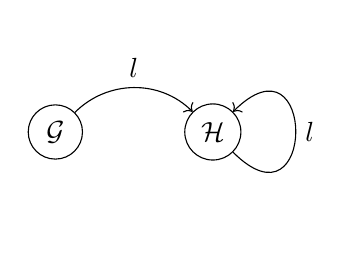
\begin{tikzpicture}
            \node[shape=circle, draw=black] (G) at (0,0) {\(\Gc\)};
            \node[shape=circle, draw=black] (H) at (2,0) {\(\Hc\)};
    
            \path [->] (G) edge[out=45, in=135] node[above] {\(l\)} (H);
            \path [->] (H) edge[out=-45, in=45, distance=15mm] node[right] {\(l\)} (H);
    
        \end{tikzpicture} 

        \caption{A graph connecting \(\Gc\) to \(\Hc\).}
    \end{figure}

    \begin{theorem}
        Let \(\Gc\) and \(\Hc\) be irreducible graphs, and \(\Kc\) be the graph connecting 
        \(\Gc\) to \(\Hc\) via \(I\) and \(J\).
        If \(\shift{\Kc}\) is irreducible, then
        \(\shift{\Gc} \subseteq \shift{\Hc}\).
    \end{theorem}

    \begin{proof}
        First, suppose that \(\shift{\Kc}\) is irreducible, and let \(u \in \Bc(\shift{\Gc})\). 
        There is a path in \(\Gc\) that presents \(u\), hence there is a path in the 
        \(\Gc\) subgraph of \(\Kc\) that presents \(u\). From the irreducibility of 
        \(\Gc\), there is a path from the terminating vertex of a path presenting 
        \(u\) to \(I\). Let \(v\) be the word such path presents and \(l\) be 
        the label of the edge connecting \(\Gc\) to \(\Hc\), so that we have 
        \(uvl \in \Bc(\shift{\Kc})\) and \(u \in \Bc(\shift{\Kc})\). As \(\shift{\Kc}\)
        is irreducible, there exists a word \(w \in \Bc(\shift{\Kc})\) such that 
        \(uvlwu \in \Bc(\shift{\Kc})\). A path presenting \(uvlwu\) must have the 
        subpath presenting \(wu\) visit vertices only from the \(\Hc\) subgraph of \(\Kc\).
        This implies that there is a path in \(\Hc\) presenting \(u\), so we have 
        \(u \in \Bc(\shift{\Hc})\) and therefore \(\Bc(\shift{\Gc}) \subseteq \Bc(\shift{\Hc})\),
        and \(\shift{\Gc} \subseteq \shift{\Hc}\) via Lemma 1.
        % Consider two words \(u, v\) from \(\Bc(\shift{\Kc})\). Suppose there is a path 
        % that presents \(u\) and ends in \(\Gc\) and a path \(\)
        %
        % Then there is always a word \(w \in \Bc(\shift{\Kc})\)
        % such that \(uwv \in \Bc(\shift{\Kc})\), as from 
        %
        % Conversely, suppose \(\shift{\Gc} \subseteq \shift{\Hc}\). Let \(u, v\) be words from \(\Bc(\shift{\Kc})\),
        % and \(\pi, \tau\) be paths presenting \(u\) and \(v\), respectivley. 
        % If \(\pi\) ends in \(\Gc\), then consider either the case where \(\tau\) starts 
        % in \(\Gc\) and the case where \(\tau\) starts in \(\Hc\).
        % In the first case, from irreducibility of \(\Gc\), there is a path 
        % connecting \(\pi\) to \(\tau\). In the second case, from the irreducibility 
        % of \(\Gc\), there is a path connecting \(\pi\) to the path starting at \(I\) and 
        % ending at \(J\) (that is, the edge connecting \(\Gc\) to \(\Hc\)). From the 
        % irreducibility of \(\Hc\), there is a path from \(J\) to the starting vertex 
        % of \(\tau\), so if \(\tau\) ends in \(\Hc\), then there is a path connecting 
        % \(\pi\) to \(\tau\). Hence, for a word \(u\) with a path ending in \(\Gc\) 
        % that presents it, then there exists a word \(w \in \Bc(\shift{\Kc})\) such 
        % that \(uwv \in \Bc(\shift{\Kc})\).
        % If \(\pi\) does not end in \(\Gc\), then it ends in \(\Hc\). From the 
        % irreducibility of \(\Hc\), there is a path connecting \(\pi\) to \(\tau\)
        % if \(\tau\) starts in \(\Hc\). If \(\tau\) started in \(\Gc\), then there is no
        % path connecting them. However, if \(\tau\) ends in \(\Hc\), then the \(\tau = \tau_1 e \tau_2\)
        % where \(\tau_1\) is a path in \(\Gc\) ending at \(I\).
        % We have \(\Lc(\tau_1) \in \Bc(\shift{\Gc})\) and hence \(\Lc(\tau_1) \in \Bc(\shift{\Hc})\)
        % since \(\shift{\Gc} \subseteq \shift{\Hc}\).
        % This means there is a path \(\tau_1'\) in \(\Hc\) that presents 
    \end{proof}

    \begin{theorem}
        Let \(\Gc\) and \(\Hc\) be irreducible, minimal, right-resolving presentations. 
        If \(\shift{\Gc} = \shift{\Hc}\), then there exists a pair
        of vertices \((I, J) \in (\Vc_\Gc \times \Vc_\Hc)\) such that both the graph connecting \(\Gc\) to \(\Hc\) via 
        \(I\) and \(J\) and the graph connecting \(\Hc\) to \(\Gc\) via \(J\) and \(I\) both 
        present irreducible shifts.

        Equivalently, if for every pair of vertices \((I, J) \in (\Vc_\Gc, \Vc_\Hc)\) 
        the graph connecting \(\Gc\) to \(\Hc\) via \(I\) and \(J\) 
        and the graph connecting \(\Hc\) to \(\Gc\) via \(J\) and \(I\)
        do not both present irreducible shifts.
    \end{theorem}

    \begin{proof}
        Suppose \(\shift{\Gc} = \shift{\Hc}\). Since \(\Gc\) and \(\Hc\) are irreducible,
        minimal, right-resolving presentations of the same shift, they must be 
        isomorphic. Let \((\partial\Phi, \Phi)\) be a graph isomorphism between them. 
        Choose an arbitrary vertex I from \(\Gc\), and then let \(\Kc\) 
        be the graph connecting \(\Gc\) to \(\Hc\) via \(I\) and \(\partial\Phi(I)\).
        Let \(f\) be the self loop on \(\partial\Phi(I)\) added in the construction of
        \(\Kc\), and \(\Hc^+\) be the \(\Hc\) of \(\Kc\) subgraph plus \(f\).
         As 
        \(\Hc\) is irreducible, then \(\Hc^+\) is irreducible. 
        It suffices to show that \(\shift{\Kc} = \shift{\Hc^+}\) to show \(\shift{\Kc}\) 
        is irreducible. 

        % Let \(u, v\) be words from \(\Bc(\shift{\Kc})\),
        % and \(\pi, \tau\) be paths presenting \(u\) and \(v\), respectivley. 
        % If \(\pi\) ends in \(\Gc\), then consider either the case where \(\tau\) starts 
        % in \(\Gc\) and the case where \(\tau\) starts in \(\Hc\).
        % In the first case, from irreducibility of \(\Gc\), there is a path 
        % connecting \(\pi\) to \(\tau\). In the second case, from the irreducibility 
        % of \(\Gc\), there is a path connecting \(\pi\) to the path starting at \(I\) and 
        % ending at \(J\) (that is, the edge connecting \(\Gc\) to \(\Hc\)). From the 
        % irreducibility of \(\Hc\), there is a path from \(J\) to the starting vertex 
        % of \(\tau\), so in total, if \(\tau\) ends in \(\Hc\), then there is a path connecting 
        % \(\pi\) to \(\tau\). Hence, for a word \(u\) with a path ending in \(\Gc\) 
        % that presents it, then there exists a word \(w \in \Bc(\shift{\Kc})\) such 
        % that \(uwv \in \Bc(\shift{\Kc})\).

        % If \(\pi\) does not end in \(\Gc\), then it ends in \(\Hc\). From the 
        % irreducibility of \(\Hc\), there is a path connecting \(\pi\) to \(\tau\)
        % if \(\tau\) starts in \(\Hc\). If \(\tau\) started in \(\Gc\), then there is no
        % path connecting \(\pi\) to \(\tau\). However, if \(\tau\) ends in \(\Hc\), then the \(\tau = \tau_1 e \tau_2\)
        % where \(\tau_1\) is a path in \(\Gc\) ending at \(I\), \(e\) is the edge connecting 
        % \(\Gc\) and \(\Hc\), and \(\tau_2\) is a path in \(\Hc\) starting at \(J\).

        Let \(u\) be a word from \(\Bc(\shift{\Kc})\), and \(\pi\) be a path that presents it.
        Without loss of generality, assume \(u\) and \(\pi\) are nonempty.
        If \(\pi\) starts in \(\Hc^+\), then \(u \in \Bc(\shift{\Hc^+})\). Otherwise, it 
        starts in \(\Gc\) and either ends in \(\Gc\) or ends in \(\Hc^+\). 
        For the case of \(\pi\) ending in \(\Gc\), then \(\Phi(\pi)\) is a path in 
        \(\Hc\) presenting \(u\), as \((\partial\Phi, \Phi)\) is a graph isomorphism,
        so \(u \in \Bc(\shift{\Hc^+})\).
        For the case of \(\pi\) ending in \(\Hc^+\), we can split 
        \(\pi\) into \(\pi=\pi_1 e \pi_2\), where \(\pi_1\) and \(\pi_2\)
        are (possibly empty) paths from \(\Gc\) and \(\Hc^+\), respectivley, and 
        \(e\) is the edge connecting \(\Gc\) and \(\Hc\). Note 
        that \(\Phi(\pi_0)\) is a path in \(\Hc\) and that it terminates
        at \(\partial\Phi(I)\) as \(\pi_0\) terminates at \(I\), assuming \(\pi_0\) is nonempty.
        From this, we have that \(\Phi(\pi_0)f\pi_1\) is path in \(\Hc^+\) that presents \(u\), 
        so \(u \in \Bc(\shift{\Hc^+})\).

        Hence, we have \(\Bc(\shift{\Kc}) \subseteq \Bc(\shift{\Hc^+})\), and from 
        the construction of \(\Kc\), we also have \(\Bc(\shift{\Hc^+}) \subseteq \Bc(\shift{\Kc})\), 
        so \(\Bc(\shift{\Kc}) = \Bc(\shift{\Hc^+})\) and \(\shift{\Kc} = \shift{\Hc^+}\). Thus,
        we have shown the graph connecting \(\Gc\) to \(\Hc\) via \(I\) and \(\partial\Phi(I)\)
        presents an irreducible shift. A similar argument can be made showing that 
        the graph connecting \(\Hc\) to \(\Gc\) via \(\partial\Phi(I)\) and \(I\) presents 
        an irreducible shift (start from ``\dots and then let \(\Kc\)'', and replace
        \(\Gc \mapsto \Hc, \Hc \mapsto \Gc, I \mapsto \partial\Phi(I), \partial\Phi(I) \mapsto I,
        \Hc^+ \mapsto \Gc^+, \Phi(\pi_0) \mapsto \Phi^{-1}(\pi_0)\)).
    \end{proof}

    \begin{theorem}
        Given an oracle for minimizing a reducible presentation, deciding 
        if two irreducible, minimal, right-resolving labeled graphs are isomorphic can be determined in polynomial time.
    \end{theorem}

    \begin{proof}
        Let the decision procedure be as follows:
        for every pair of vertices
        \((I, J) \in (\Vc_\Gc \times \Vc_\Hc)\) between the graphs,
        construct and set \(\Gc_I\to\Hc_J\) as the graph connecting \(\Gc\) to \(\Hc\)
        via \(I\) and \(J\), and similarly, construct and set \(\Hc_J \to \Gc_I\) as the graph connecting 
        \(\Hc\) to \(\Gc\) via \(J\) and \(I\). Then,
        using the oracle, minimize \(\Gc_I \to \Hc_J\) and check if it is strongly connected (that is, irreducible),
        and if so, then from Theorem 2, we know we can 
        set \(\shift{\Gc} \subseteq \shift{\Hc}\) to be true.
        Similary, minimize \(\Hc_J \to \Gc_I\) and check if it is strongly connected, and 
        if so, set \(\shift{\Hc} \subseteq \shift{\Gc}\) to be true.
        If at any point both \(\shift{\Gc} \subseteq \shift{\Hc}\) and \(\shift{\Hc} \subseteq \shift{\Gc}\)
        are set to true, then \(\shift{\Gc} = \shift{\Hc}\) and thus can conclude \(\Gc \cong \Hc\) (as 
        \(\Gc\) and \(\Hc\) are unique, minimal, and irreducible presentations). If you find that 
        after every pair of verticies that one or both  
        of \(\shift{\Gc} \subseteq \shift{\Hc}\) and \(\shift{\Hc} \subseteq \shift{\Gc}\)
        were not set to true, then we have that for all pairs of verticies,
        the presentations of the pair of graphs constructed were not both 
        irreducible, as if they were, then both \(\shift{\Gc} \subseteq \shift{\Hc}\)
        and \(\shift{\Hc} \subseteq \shift{\Gc}\) would be true, so via Theorem 3, we have that \(\shift{\Gc} \neq \shift{\Hc}\)
        and can conclude \(\Gc \ncong \Hc\) (as again, \(\Gc\) and \(\Hc\) are irreducible, minimal, right-resolving 
        graphs).
        
        The worst case runtime of the decision procedure is if \(\Gc \ncong \Hc\),
        as we minimize and check strongly connected-ness twice 
        (of a graph that is potentially the size of both \(\Gc\) and \(\Hc\))
        for each pair of verticies, so the runtime is \(O((V+E)\cdot V^2)\),
        where \(V\) is the number of verticies of one graph and \(E\)
        is the number of edges of one graph.
    \end{proof}

\newpage

\section{Graph isomorphisms}

\begin{definition}
    An \term{undirected graph} is a pair \(G = (V, E)\), where \(V\) is a 
    finite set of vertices and \(E \subseteq V \times V\) is a symmetric and irreflexive relation
    on \(V\).
\end{definition}

\begin{definition}
    Given undirected graphs \(G = (V_G, E_G)\) and \(H = (V_H, E_H)\), an isomorphism from \(G\) to \(H\)
    is a bijection \(\varphi : V_G \to V_H\) such that for all \(I, J \in V_G\), 
    \((I, J) \in E_G\) if and only if \((\varphi(I), \varphi(J)) \in E_H\). If there is 
    and isomorphism from \(G\) to \(H\), then we say \(G\) and \(H\) are isomorphic.

    Given labeled graphs \(\Gc\) and \(\Hc\), an isomorphism from \(\Gc\) to \(\Hc\) 
    is a pair of bijections \(\partial\Phi : \Vc_\Gc \to \Vc_\Hc\) and \(\Phi : \Ec_\Gc \to \Ec_\Hc\)
    such that for all \(e \in \Ec_\Gc\), \(i_\Hc(\Phi(e)) = \partial\Phi(i_\Gc(e))\), 
    \(t_\Hc(\Phi(e)) = \partial\Phi(t_\Gc(e))\), and \(\Lc_\Hc(\Phi(e)) = \Lc_\Gc(e)\).
\end{definition}

\begin{definition}
    Define the decision problem \(\GI\) to be the set of all pairs of isomorphic undirected graphs:
    \[\GI \triangleq \{ \langle G, H \rangle : G \text{ and } H \text{ are isomorphic undirected graphs} \}\]
    Similary, define the decision problem \(\LGI\) to be the set of all pairs of isomorphic labeled graphs:
    \[\LGI \triangleq \{ \langle \Gc, \Hc \rangle : \Gc \text{ and } \Hc \text{ are isomorphic labeled graphs} \}\]
\end{definition}

\begin{definition}
    Let \(A\) be some decision problem. We say \(A\) is \term{\(\GI\)-hard} if \(\GI\) is polynomial-time Turing reducible 
    to \(A\). We say \(A\) is \term{\(\GI\)-complete} if \(A\) is \(\GI\)-hard and \(A\) is polynomial-time
    Turing reducible to \(\GI\).
\end{definition}

\begin{theorem}
    \(\LGI\) is \(\GI\)-hard.
\end{theorem}

\begin{proof}
    % Let \(\Gc\) and \(\Hc\) be labeled graphs. Construct the undirected graph \(G\),
    % setting \(V_G \triangleq \Vc_\Gc\) and setting \(E_G\) 
    % to be the reflexive closure of \(\{ (I, J) \in \Vc_\Gc \times \Vc_\Gc : I \neq J, i(e) = I \text{ and } t(e) = J \text{ for some } e \in \Ec_\Gc \}\).
    % Construct the undirected graph \(H\) in a similar fashion. 
    
    % Suppose \((\partial\Phi, \Phi)\) is an isomorphism from \(\Gc\) to \(\Hc\), then \(\partial\Phi\)
    % is an isomorphism from \(G\) to \(H\). Let \(I, J \in V_G\). If \((I, J) \in E_G\), 
    % then \(\partial\Phi(I)\)

    First, we will show that \(\LGI\) is \(\GI\)-hard. Let 
    \(G\) and \(H\) be undirected graphs. Construct the labeled graph \(\Gc\) 
    with \(\Vc_\Gc \triangleq V_G\), \(\Ec_\Gc \triangleq E_G\) and for all \(I, J \in \Ec_\Gc\),
    \(i_\Gc(I, J) \triangleq I\), \(t_\Gc(I, J) \triangleq J\), and \(\Lc_\Gc(I, J) \triangleq \ell\). 
    Construct the labeled graph \(\Hc\) in a similar fashion. Obviously, this construction can be done in polynomial-time with respect 
    to the size of \(G\) and \(H\).

    Suppose \(\varphi\) is an isomorphism from \(G\) to \(H\). Define the map 
    \(\partial\Phi : \Vc_\Gc \to \Vc_\Hc\) with \(\partial\Phi(I) \triangleq \varphi(I)\) for \(I \in \Vc_\Gc\) 
    and \(\Phi : \Ec_\Gc \to \Ec_\Hc\) with \(\Phi(I, J) \triangleq (\varphi(I), \varphi(J))\)
    for \(I, J \in \Ec_\Gc\).
    % then we can show the maps 
    % \(\partial\Phi \triangleq \varphi\) and \(\Phi \triangleq \varphi \times \varphi\)
    % \footnote{
    %     For functions \(f: A \to C\) and \(g: B \to D\), define the product \(f \times g : A \times B \to C \times D\)
    %     as \((f \times g)(a, b) \triangleq (f(a), g(b))\).
    % }
    % are an isomorphism from \(\Gc\) to 
    % \(\Hc\).
    Let \((I, J) \in \Ec_\Gc\). Then, 
    \begin{align*}
        \partial\Phi(i_\Gc(I, J)) &= \partial\Phi(I) \\ 
        &= \varphi(I) \\
        &= i_\Hc(\varphi(I), \varphi(J)) \qquad (\star)\\ 
        &= i_\Hc(\Phi(I, J)),
    \end{align*}
    and \((\star)\) is well-defined as \((I, J) \in \Ec_\Gc = E_G\) if and only if \((\varphi(I), \varphi(J)) \in E_H = \Ec_\Hc\).
    A similar deduction can be used to show \(\partial\Phi(t_\Gc(I, J)) = t_\Hc(\Phi(I, J))\). 
    As \(\varphi\) is a bijection from \(V_G\) to \(V_H\), then \(\partial\Phi\) is a 
    bijection from \(\Vc_\Gc\) to \(\Vc_\Hc\). One can check that for \(\Phi^{-1}(I, J) \triangleq (\varphi^{-1}(I), \varphi^{-1}(J))\),
    \(\Phi^{-1} \circ \Phi = id_{\Ec_\Gc}\) and \(\Phi \circ \Phi^{-1} = id_{\Ec_\Hc}\) 
    so \(\Phi\) is a bijection from \(\Gc\) to \(\Hc\). Hence, \((\partial\Phi, \Phi)\) is an 
    isomorphism from \(\Gc\) to \(\Hc\).

    Conversely, suppose \((\partial\Phi, \Phi)\) is an isomorphism from \(\Gc\) to \(\Hc\). Define 
    \(\varphi : V_G \to V_H\) with \(\varphi(I) \triangleq \partial\Phi(I)\) for \(I \in V_G\). 
    Note that for \((I, J) \in \Ec_\Hc\), \((I, J) = (i_\Hc(I,J), t_\Hc(I, J))\). If \((I, J) \in E_G\),
    then 
    \begin{align*}
        i_\Hc(\Phi(I, J)) &= \partial\Phi(i_\Gc(I, J)) \\ 
        &= \partial\Phi(I) \\ 
        t_\Hc(\Phi(I, J)) &= \partial\Phi(t_\Gc(I, J)) \\ 
        &= \partial\Phi(J),
    \end{align*}
    so \(\Phi(I, J) = (i_\Hc(\Phi(I, J)), t_\Hc(\Phi(I, J))) = (\partial\Phi(I), \partial\Phi(J)) = (\varphi(I), \varphi(J))\).
    Therefore, as \(\Phi(I, J) \in \Ec_\Hc = E_H\), then \((\varphi(I), \varphi(J)) \in E_H\).
    Simlarly, note that for \(I, J \in E_\Gc\), \((I, J) = (i_\Gc(I, J), t_\Gc(I, J))\). If 
    \((\varphi(I), \varphi(J)) \in E_H\), then 
    \begin{align*}
        i_\Hc(\Phi(I, J)) &= \partial\Phi(i_\Gc(I, J)) \\ 
        &= \partial\Phi(I) \\ 
        t_\Hc(\Phi(I, J)) &= \partial\Phi(t_\Gc(I, J)) \\ 
        &= \partial\Phi(J),
    \end{align*}
    
\end{proof}



\end{document}